\subsection{Separability is Equivalent to Regular Colourability}

We start by showing that the "separability problem" in terms of arbitrary "recognizable relations" is equivalent, under polynomial time reductions, 
to the "regular colourability problem". To make our statement precise, we need some terminology introduced below. 
\AP
Let $\intro*\kREC$ be the class of languages expressed by unions of products of $k$ regular languages which form a partition, that is (in the binary case), relations of the form $(L_{i_1} \times L_{j_1}) \cup \dotsb \cup (L_{i_\ell} \times L_{j_\ell})$, with $i_1,j_1,\hdots,i_\ell, j_\ell \in \lBrack 1,k \rBrack$, for some regular partition $L_1, \dotsc, L_{k}$ of $\Sigma^*$ and $\ell \in \N$.
\AP
Note that $\REC = \bigcup_k \kREC$.
\AP%
Let us denote by $\intro*\Id$ the identity relation (on any implicit alphabet). Observe that $\Id$ is "automatic" but not "recognizable".

\begin{theorem}
    \AP\label{thm:reg-colourability-equiv-separability}
    There are polynomial-time reductions: 
    \begin{enumerate}
        \item from the "$\REC$-separability problem" to the "regular colourability problem"; 
        \item from the "regular colourability problem" to the "$\REC$-separability problem"; and
        \item from the "$k$-regular colourability problem" to the $\kREC$-"separability problem", for every $k > 0$.
    \end{enumerate}
    Further, the last two reductions are so that the second relation in the instance of the "separability problem" is the identity $\Id$.
\end{theorem}
   
\begin{proof}
   We start with the last two reductions.
    Given an "automatic graph" $\AutGraph{L}{E}$ over an alphabet $\Sigma$, consider the instance $R_1,R_2$ for the $\REC$-"separability problem", where 
    $R_1 = E$ and $R_2 = \Id$. 
    %
    If $\AutGraph{L}{E}$ is "$k$-regular colourable" via the colouring $V_1, \dotsc, V_k$ then the $\kREC$ relation
    $\bigcup_{i \neq j} V_i \times V_j$ separates $R_1$ and $R_2$.
    %
    Conversely, if a $\kREC$ relation $R \subseteq \Sigma^* \times \Sigma^*$ on the partition $V_1 \dcup \dotsb \dcup V_k = \Sigma^*$ separates $R_1$ and $R_2$, then $\bigcup_{i \neq j} V_i \times V_j$ also separates $R_1$ and $R_2$, and this implies that $V_1, \dotsc, V_k$ is a $k$-colouring for $\AutGraph{\Sigma^*}{E}$.
%\end{proof}

\AP For the first reduction, let us introduce some terminology.
Given two relations $R_1,R_2$ over $\Sigma^*$, say that $u \in \Sigma^*$ is ""compatible"" with
$u' \in \Sigma^*$ when for all words $v \in \Sigma^*$:
\begin{center}
    \intro*\compL: $(u,v) \in R_1 \Rightarrow (u',v) \not\in R_2$%
    ,\hphantom{\quad and \quad}
    \intro*\compR: $(v,u) \in R_1 \Rightarrow (v,u') \not\in R_2$,\\
    \intro*\compLpr: $(u',v) \in R_1 \Rightarrow (u,v) \not\in R_2$%
    \hphantom{,}\quad and \quad
    \intro*\compRpr: $(v,u') \in R_1 \Rightarrow (v,u) \not\in R_2$.
\end{center}
\AP
Define the ""incompatibility graph"" $\intro*\incompGraph{R_1}{R_2}$
as the graph whose vertices are all words of $\Sigma^*$,
and with an edge from $u$ to $v$ whenever $u$ is not "compatible" with $v$.
Note that $\incompGraph{R}{\Id}$ is exactly the graph $\AutGraph{\Sigma^*}{R}$.

\begin{example}
    \AP\label{ex:equal-length-plusone}%
    \begin{marginfigure}%
        \centering
        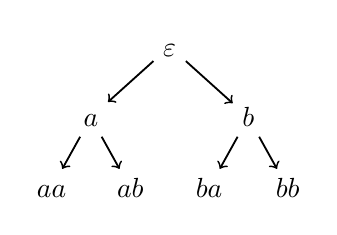
\begin{tikzpicture}
            \tikzset{
	level distance=.9cm,
	level 1/.style={sibling distance=2cm},
	level 2/.style={sibling distance=1cm},
	level 3/.style={sibling distance=.5cm},
	edge from parent/.style={draw, ->, line width=.66pt}
}

\node (t) {$\varepsilon\vphantom{b}$}
	child {node {$a\vphantom{b}$}
		child {node {$aa\vphantom{b}$}
		}
		child {node {$ab$}
		}
	}
	child {node {$b$}
		child {node {$ba$}
		}
		child {node {$bb$}
		}
	};
        \end{tikzpicture}
        \caption{\AP\label{fig:equal-length-plusone-relation}%
            The relation $R_2$ of \Cref{ex:equal-length-plusone},
            restricted to words of length at most 2.
        }
    \end{marginfigure}%
    \begin{marginfigure}%
        \centering
        \begin{tikzpicture}
            \tikzset{
	level distance=.9cm,
	level 1/.style={sibling distance=2.8cm},
	level 2/.style={sibling distance=1.4cm},
	level 3/.style={sibling distance=.7cm},
	edge from parent/.style={}
}

% Coloring
\fill[rounded corners, fill=cBlue, opacity=.5]
	(-2.5,-2.05) rectangle (2.5,-1.57)
	(-.3,-0.25) rectangle (.3,0.23);
\fill[rounded corners, fill=cYellow, opacity=.5]
	(-1.65,-1.15) rectangle (1.65,-0.67);
% Tree
\node (eps) {$\varepsilon\vphantom{b}$}
	child {node (a) {$a\vphantom{b}$}
		child {node (aa) {$aa\vphantom{b}$}
		}
		child {node (ab) {$ab$}
		}
	}
	child {node (b) {$b$}
		child {node (ba) {$ba$}
		}
		child {node (bb) {$bb$}
		}
	};
\draw[<->] (eps) edge (a)
	(eps) edge (b)
	(a) edge (aa)
	(a) edge (ab)
	(a) edge (ba)
	(a) edge (bb)
	(b) edge (aa)
	(b) edge (ab)
	(b) edge (ba)
	(b) edge (bb);
        \end{tikzpicture}
        \caption{\AP\label{fig:equal-length-plusone-incompatibility}%
            Incompatibility graph $\incompGraph{R_1}{R_2}$ and its "2-regular colouring".%
        }
    \end{marginfigure}%
    Let $\Sigma = \{a,b\}$, $R_1$ be the equal-length relation,
    and
    \[
        R_2 = \{(u, ua) \mid u \in \Sigma^*\} \cup \{(u, ub) \mid u \in \Sigma^*\}.
    \]
    Then, $u$ is "incompatible" with $u'$ if $|u| = |u'|+1$ (this is given by \compL~or \compR),
    or if $|u'| = |u|+1$ (this is given by \compLpr~or \compRpr).
    $R_2$ and the "incompatibility graph" are depicted in \Cref{fig:equal-length-plusone-relation,fig:equal-length-plusone-incompatibility}.
    
    Note that $R_1$ and $R_2$ are separable by the "recognizable" relation
    $S$ consisting of all pairs $(u,v)$ such that $|u|$ and $|v|$ have the same parity.
    Moreover, $\incompGraph{R_1}{R_2}$ is "2-regular colourable", the two colours being
    the words of even and odd length.
\end{example}

\begin{lemma}
    \AP\label{lem:incomp-is-automatic}
    If $R_1$ and $R_2$ are "automatic", then so is $\incompGraph{R_1}{R_2}$.
    Moreover, we can build an automaton for $\incompGraph{R_1}{R_2}$ in polynomial time in the size of the automata for $R_1$ and $R_2$.
\end{lemma}

\begin{proof}
    By definition, the "incompatibility relation" $\incompGraph{R_1}{R_2}$ can be written as
	$R_{\neg\compL} \cup R_{\neg\compLpr} \cup R_{\neg\compR} \cup R_{\neg\compRpr}$, where:
	\begin{align*}
        R_{\neg\compL} &\defeq \big\{ (u,u') \in \Sigma^* \times \Sigma^* \;\big\vert\; \exists v \in \Sigma^*,\; (u,v) \in R_1 \land (u',v) \in R_2 \big\} \text{,}\\
        R_{\neg\compLpr} &\defeq \big\{ (u,u') \in \Sigma^* \times \Sigma^* \;\big\vert\; \exists v \in \Sigma^*,\; (u',v) \in R_1 \land (u,v) \in R_2 \big\} \text{,}\\
        R_{\neg\compR} &\defeq \big\{ (u,u') \in \Sigma^* \times \Sigma^* \;\big\vert\; \exists v \in \Sigma^*,\; (v,u) \in R_1 \land (v,u') \in R_2 \big\} \text{, and}\\
        R_{\neg\compRpr} &\defeq \big\{ (u,u') \in \Sigma^* \times \Sigma^* \;\big\vert\; \exists v \in \Sigma^*,\; (v,u') \in R_1 \land (v,u) \in R_2 \big\}
    \end{align*}
    % % \end{itemize}
    % \begin{itemize}
    %     \item $\neg$\compL:  $(u,v) \in R_1$ and $(u',v) \in R_2$, or
    %     \item $\neg$\compLpr: $(u',v) \in R_1$ and $(u,v) \in R_2$, or
    %     \item $\neg$\compR: $(v,u) \in R_1$ and $(v,u') \in R_2$, or
    %     \item $\neg$\compRpr: $(v,u') \in R_1$ and $(v,u) \in R_2$.
    % \end{itemize} 
    Observe that starting from automata for $R_1$ and $R_2$, then for each
	of the relation $R_{\neg\compL}$, $R_{\neg\compLpr}$, $R_{\neg\compR}$ or $R_{\neg\compRpr}$, we can build an automaton recognizing them
	using a product construction, which can be implemented in polynomial time.
    % as follows:
    % \begin{itemize}
    %     \item its states are $Q_1 \times Q_2$;
    %     \item for each transition $q_1 \xrightarrow{(a,b)} q'_1$ in $\+A_1$
    %         and each transition $q_2 \xrightarrow{(c,b)} q'_2$ in $\+A_2$,
    %         put a transition $(q_1,q_2) \xrightarrow{(a,c)} (q'_1,q'_2)$,
    %         with $a,b,c \in \A\cup\{\bot\}$;\footnote{Potentially, this
    %         could produced transition labelled by $(\bot,\bot)$: we can get rid of those
    %         using the standard elimination of $\varepsilon$-transitions.}
    %     \item a state $(q_1,q_2)$ is accepting if $q_1$ and $q_2$ are accepting
    %         in $\+A_1$ and $\+A_2$, respectively.
    % \end{itemize}
    It then follows that we can build a polynomial automaton recognizing
    $\incompGraph{R_1}{R_2}$.
\end{proof}

%\begin{proposition}
%    \AP\label{prop:sep-to-col-reduction}
%    There is a polynomial-time reduction
%    from the $\REC$-"separability problem" to the 
%    "regular colourability problem" on "automatic graphs".
%\end{proposition}

%\begin{proof}
    \AP Given an instance $(R_1,R_2)$ of the "separability problem", we
    reduce it to the "regular colourability problem" on its "incompatibility graph" $\incompGraph{R_1}{R_2}$.

    \proofcase{Left-to-right implication:} 
   Assume that there exists $S$ in $\kREC$ that "separates" $R_1$ from $R_2$.
   %, where each $A_i$ and $B_i$ is regular.
    Then $S$ can be written as $(A_{i_1}\times A_{j_1}) \cup \cdots \cup (A_{i_\ell}\times A_{j_\ell})$, 
    where $(A_1,\hdots,A_k)$ is a partition of $\Sigma^*$ in $k$ regular languages.
   We define the colour of a word $u \in \Sigma^*$ as the unique $i \in \lBrack 1,k \rBrack$
    "st" $u \in A_i$. In other words, the colouring is simply $(A_1,\hdots,A_k)$. 

    This is indeed a proper colouring: if $u$ and $u'$ have the same colour,
    we claim that $u$ is "compatible" with $u'$. Indeed, take any $v \in \Sigma^*$: if $(u,v) \in R_1$,
    then $(u,v) \in S$, so $(u,v) \in A_{i_m}\times A_{j_m}$ for some $m$. But since $u$ has the same colour 
    as $u'$, the fact that $u \in A_{i_m}$ implies $u' \in A_{i_m}$, and hence 
    $(u',v) \in A_{i_m}\times A_{j_m}\subseteq S$.
    But $S$ separates $R_1$ from $R_2$, and therefore $(u',v) \not\in R_2$. This tells us that \compL\ holds. 
    The other conditions hold by symmetry.
    We conclude that $(A_1,\hdots,A_k)$ defines
    a proper colouring of $\incompGraph{R_1}{R_2}$, and this colouring, with $k$ colours, is 
    "regular@regular colouring" since the $A_i$'s are regular languages by definition.

    \proofcase{Right-to-left implication:} Assume that $\incompGraph{R_1}{R_2}$ is finitely colourable, say by
    $(A_1,\hdots,A_k)$. Then let $S$ be the union of all $S_i$'s where
    \begin{align*}
        S_{i} & \defeq \{(u,v) \mid u \in A_i \text{ and } (u',v) \in R_1 \text{ for some } u' \in A_i \}\\
&         \hphantom{\defeq~}\cup \{(u,v) \mid v \in A_i \text{ and } (u,v') \in R_1 \text{ for some } v' \in A_i \}.  
    \end{align*}
    Since $(A_1,\hdots,A_k)$ covers every node of $\incompGraph{R_1}{R_2}$, we get $R_1 \subseteq S$.
    Moreover, we claim that $R_2 \cap S = \emptyset$. Indeed, if $(u,v) \in S$,
    then $(u,v) \in S_{i}$ for some $i,j$. It either means that \proofcase{1}
    $(u',v) \in R_1$ for some $u' \in A_i$, or \proofcase{2} $(u,v') \in R_2$
    for some $v' \in A_i$. In case \proofcase{1}, the fact that $u \in A_i$ implies that $u$ and $u'$
    have the same colour. Thus, $u$ must be "compatible" with $u'$ and hence
    $(u,v) \not\in R_2$ using \compLpr. The other case is symmetric.
    Therefore, $(u,v) \not\in R_2$, and thus $S$ separates $R_1$ from $R_2$.

    Finally,  $S$ is "recognizable"; in fact, 
    $S = \bigcup_{i=1}^k \bigl( A_i \times R_1[A_i] \bigr) \cup \bigl( R_1^{-1}[A_i] \times A_i \bigr)$, 
    where for any set $X \subseteq \Sigma^*$ we define $R_1[X]$ (resp. $R_1^{-1}[X]$) as the set
    of $v\in \Sigma^*$ (resp. $u \in \Sigma^*$) such that $(u,v) \in R_1$ for some $u \in X$
    (resp. $v\in X$).
    Hence, $R_1$ and $R_2$ are $\REC$-"separable". 
\end{proof}

It is not known to date whether the "regular colourability problem" is decidable, and hence 
the same holds for the $\REC$-"separability problem"
in light of the previous theorem. This is due to the fact that there are no known characterizations of when an "automatic graph" is finitely colourable. 
In spite of this, we believe that the connection between separability and finite colourability is of interest, as it provides us with a way to define and study meaningful 
restrictions of our problems. The first such restriction corresponds to the "$k$-regular colourability problem" for "automatic graphs", which we study in the next section. 
